% https://tex.stackexchange.com/questions/158585/draw-3d-intersecting-surfaces
\documentclass{article}
\usepackage{tikz}
\usetikzlibrary{intersections}

\begin{document}

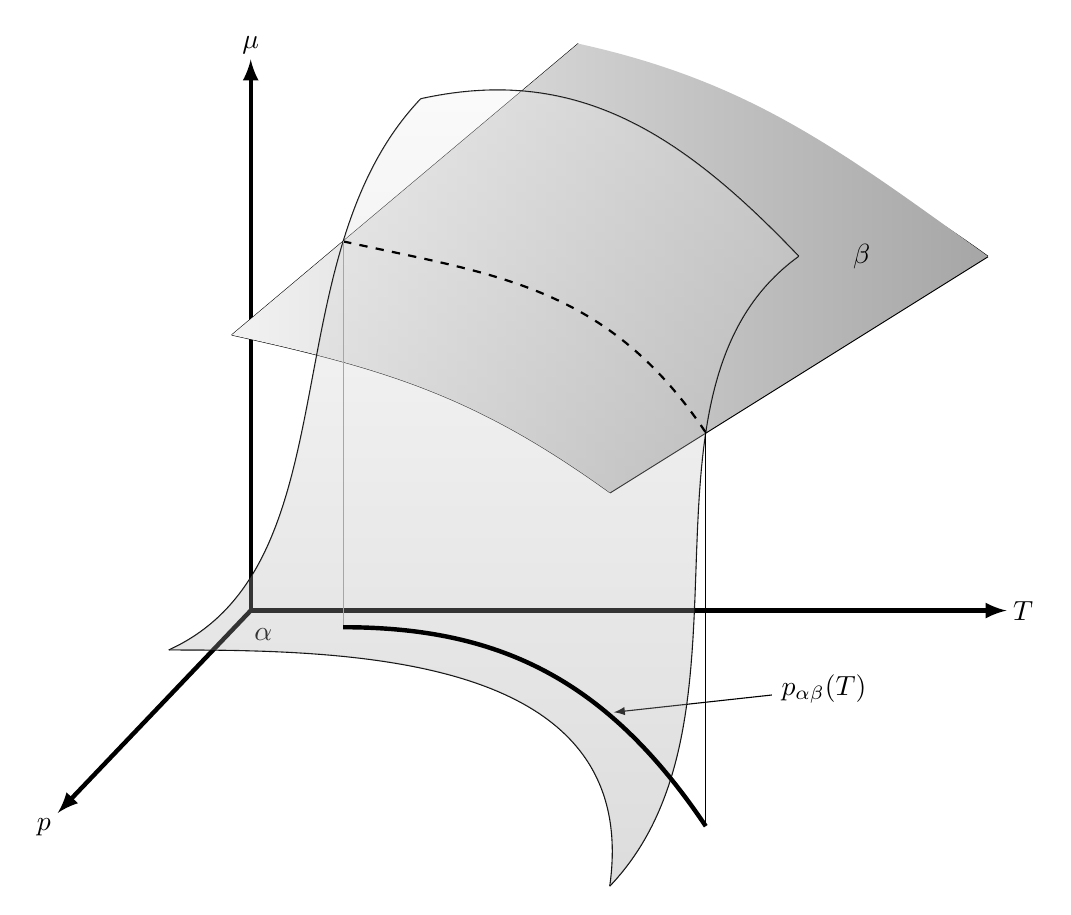
\begin{tikzpicture}[xscale=0.8,>=latex]
% axis
\draw[ultra thick,->] (0.3,-3.5) -- +(0,7) node[yshift=5pt] {$\mu$};
\draw[ultra thick,->] (0.3,-3.5) -- +(220:4) node[yshift=-5pt,xshift=-5pt] {$p$};
\draw[ultra thick,->] (0.3,-3.5) -- +(12,0) node[xshift=6pt] {$T$};

% border of the surface1
\path[draw,name path=border1] (0,0) to[out=-10,in=150] (6,-2);
% border of the surface1
\path[draw,name path=border2] (12,1) to[out=150,in=-10] (5.5,3.2);
% border of the surface1
\draw[draw,thick,name path=line1] (6,-2) -- (12,1);
% border of the surface1
\path[draw,name path=line2] (5.5,3.7) -- (0,0);
% draw the surface1
\shade[left color=gray!10,right color=gray!70] 
  (0,0) to[out=-10,in=150] (6,-2) -- 
  (12,1) to[out=150,in=-10] (5.5,3.7) -- cycle;

% border of the surface2
\path[draw,name path=border3] (-1,-4) to[out=20,in=220] (3,3);
% border of the surface2
\path[draw,name path=border4] (6,-7) to[out=40,in=210] (9,1);
% border of the surface2
\path[draw,name path=border5] (-1,-4) to[out=0,in=80] (6,-7);
% border of the surface2
\path[draw,name path=border6] (3,3) to[out=10,in=140] (9,1);

% labels
\node at (0.5,-3.8) {$\alpha$};
\node at (10,1) {$\beta$};
\node at (9.4,-4.5) (label) {$p_{\alpha\beta}(T)$};
\draw[->] (label) -- +(185:3.35);

% draw the surface2
\shade[top color=gray!10,bottom color=gray!90,opacity=.30] 
  (-1,-4) to[out=20,in=220] (3,3)  to[out=10,in=140] (9,1)
 to[out=210,in=40] (6,-7) to[out=80,in=0] (-1,-4);

% intersection points
\path[name intersections={of=border3 and line2,by={a}}];
\path[name intersections={of=border4 and line1,by={b}}];

% intersection of the surfaces
\draw[thick,dashed] (a) to[out=-10,in=130] (b);

% proyections of the intersection points
\draw[help lines,gray!70] (a) -- +(0,-4.9) coordinate (proy1);
\draw (b) -- +(0,-5) coordinate (proy2);

% proyection of the intersection path
\draw[ultra thick] (proy1) to[out=0,in=130] (proy2);

\end{tikzpicture}

\end{document}